% Author: Izaak Neutelings (May 2018)
% Inspiration: https://tex.stackexchange.com/questions/113900/draw-polarized-light
\documentclass[border=10pt,tikz]{standalone}
\usepackage{amsmath} % for \text
\usepackage{tikz}
\usepackage{physics}
\tikzset{>=latex} % for LaTeX arrow head
\usepackage{xcolor}
\usepackage{amsmath}
\colorlet{myblue}{black!40!blue}
\colorlet{myred}{black!40!red}
\colorlet{vcol}{green!50!black}
\colorlet{Ecol}{orange!90!black}
\colorlet{EVcol}{orange!80!black!60}
\colorlet{Bcol}{violet!90}
\begin{document}

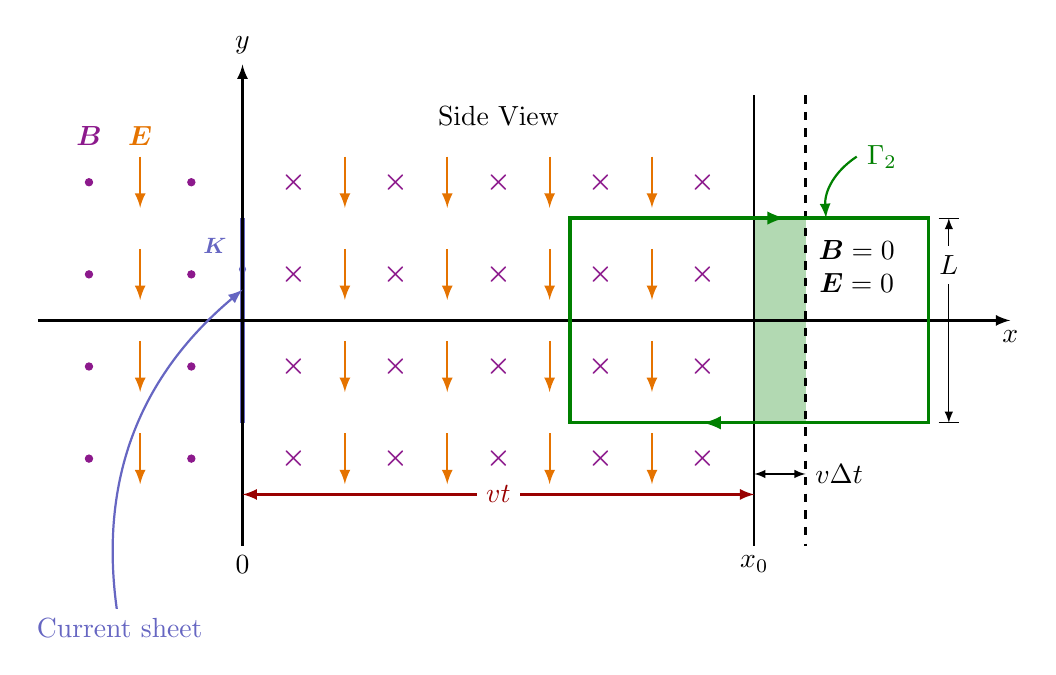
\begin{tikzpicture}[scale=1.3]
    \begin{scope}

        \foreach \x in {-1,-2}
        {
            \foreach \y in {1.35, 0.45, -0.45, -1.35}
            {
                \filldraw[Bcol] ({\x}, {\y}) circle (1pt);
            }
        }

        \foreach \x in {0,...,4}
        {
            \foreach \y in {1.35, 0.45, -0.45, -1.35}
            {
                \node[color=Bcol] at ({\x}, {\y}) {$\boldsymbol{\times}$};
            }
        }

        \foreach \x in {-1.5, 0.5, 1.5, 2.5, 3.5}
        {
            \draw[color=Ecol, thick, ->] ({\x}, 1.6) -- ({\x}, 1.1);
            \draw[color=Ecol, thick, ->] ({\x}, 0.7) -- ({\x}, 0.2);
            \draw[color=Ecol, thick, ->] ({\x}, -0.2) -- ({\x}, -0.7);
            \draw[color=Ecol, thick, ->] ({\x}, -1.1) -- ({\x}, -1.6);
        }

        \filldraw[vcol!30] (4.5, -1) rectangle (5, 1);
        \draw [dashed] (-0.5, -1.7) -- (-0.5, 1.7);
        \draw [line width=2, myblue!60] (-0.5, 1) node [yshift=-10, xshift=-10, scale=0.8] {$\boldsymbol{K}$}-- (-0.5, -1);
        \fill [myblue!60] (-0.5, 0.5) circle (1pt);
        \draw [thick, ->] (-0.5, -2.2) node [below] {$0$}-- (-0.5, 2.5) node [above] {$y$};
        \draw [thick, ] (4.5, 2.2) -- (4.5, -2.2) node [below] {$x_0$} ;
        \draw [thick, dashed] (5, 2.2) -- (5, -2.2) ;
        \draw [<->]  (4.5, -1.5) -- (5, -1.5) node [right] {$v\Delta t$};
        \draw [<->, thick, myred,] (-0.5, -1.7) -- (4.5, -1.7) node [midway, fill=white]  {$vt$};
        \draw [ thick, ->] (-2.5, 0) -- (7., 0) node [ below] {$x$};


        \draw[myblue!60, thick, ->] (-1.7, -3.0) node[fill=white] {Current sheet} to[bend left=30] (-0.5, 0.3);

        \draw [vcol, very thick, ->] (4, 1) -- (4.8, 1);
        \draw [vcol, very thick, <-] (4, -1) -- (4.8, -1);
        \draw [vcol, very thick] (2.7, 1) -- (6.2, 1) -- (6.2, -1) -- (2.7, -1) -- cycle;
     
        \draw[vcol, thick, ->] (5.5, 1.6) node[right, fill=white] {$\Gamma_2$} to[bend right=30] (5.2, 1);
        \node [] at(5.5, 0.5) {$\begin{array}{c} \boldsymbol{B}=0\\ \boldsymbol{E}=0 \end{array}$};

        \draw [] (6.3, 1) -- (6.5, 1); 
        \draw [] (6.3, -1) -- (6.5, -1); 
        \draw [<->] (6.4, -1) -- (6.4, 1) node [midway, yshift=20, fill=white] {$L$};
        \node [Bcol] at (-2, 1.8) {$\boldsymbol{B}$}; 
        \node [Ecol] at (-1.5, 1.8) {$\boldsymbol{E}$}; 
        \node [] at (2, 2) {Side View};
    \end{scope}

    

\end{tikzpicture}
\end{document}